\documentclass[onlymath]{beamer}
\usepackage{fontspec}
\usepackage{xunicode,xltxtra}
\usepackage{polyglossia}
\usepackage{xltxtra}
\usepackage{fancybox}
\usepackage{graphicx}

\usepackage{tikz}
\usetikzlibrary{calc}
\tikzset{tight/.style={inner sep=2pt}}

\usepackage{listings}
\lstset{language=C, basicstyle=\ttfamily, escapechar=|, frame=single}
\lstdefinelanguage{gdb}
{morekeywords={run,break,info,thread,set,print}}
\lstdefinestyle{session}
{frameround=tttt}
\lstdefinestyle{gdbsession}
{language=gdb,style=session}

\newcommand\tw\textwidth
\newcommand\neword\emph
\newcommand\code\texttt
\newcommand{\cenfig}[2]{\begin{figure}\centering\includegraphics[scale=#1]{#2}
  \end{figure}}
  
\usefonttheme{professionalfonts}
\usetheme[secheader]{Boadilla}
\usecolortheme{whale}

\setsansfont[Mapping=tex-text]{Myriad Pro}
\setmonofont[Mapping=tex-text]{DejaVu Sans Mono}
\setmainlanguage{russian}

\title{GDB, Emacs и Google Summer of Code }
\author{Дмитрий Джус}
\institute{МГТУ им. Н.Э.Баумана}
\date{2009}

\begin{document}

\begin{frame}
  \titlepage
\end{frame}

\begin{frame}
  \frametitle{План}
  \tableofcontents
\end{frame}

\section{GDB}

\begin{frame}
  \frametitle{Что такое отладчик}
  \begin{itemize}
  \item Debugger помогает избавиться от багов
  \item Стандартные функции отладчика
    \begin{itemize}
    \item Пошаговое исполнение программы
    \item Условный останов программы
    \item Просмотр и изменение значений переменных, памяти,
      регистров
    \item Изучение стека, нитей и дизассемблированного кода
    \end{itemize}
  \end{itemize}
\end{frame}

\begin{frame}
  \frametitle{GNU Debugger — свободный отладчик}
  \begin{columns}
    \column{.3\textwidth}
    \cenfig{0.5}{archer.jpg}
    \column{.7\textwidth}

  \begin{itemize}
  \item Переносимый отладчик для различных языков, включая C, C++ и Fortran
  \item Разработка начата rms в 1986 году в рамках проекта GNU и ныне
    продолжается силами сообщества при поддержке крупных компаний
  \item Стандартный отладчик для многих современных Unix-систем
  \item Используется в качестве компонента для ряда интегрированных
    сред разработки
  \item Поддержка удалённой отладки
  \item Различные интерфейсы (CLI для ручной работы, Machine Interface
    для IDE)
  \end{itemize}
\end{columns}
\end{frame}

\begin{frame}
  \frametitle{Новые возможности в GDB 7.0}
  \begin{itemize}
  \item Безостановочная отладка многопоточных приложений
  \item Поддержка Python в качестве языка расширения
  \item Обратимая отладка
  \end{itemize}
\end{frame}

\begin{subsection}{Отладка в режиме нон-стоп}
\begin{frame}
  \frametitle{Зачем нужна безостановочная отладка}
  \begin{itemize}
  \item Многопоточные приложения — тренд
  \item Нужно обеспечить недеструктивный контроль: отлаживать только
    ту нить, в которой проблемы
  \end{itemize}
\end{frame}

\begin{frame}[fragile]
  \frametitle{pthread.c}
  \begin{itemize}
  \item Запускаем пять нитей, одна из которых выполняет \code{f2()}
\begin{lstlisting}
for (i = 0; i < 5; i++)
{
    pthread_create(&threads[i],
                   NULL, 
                   ((i + 1) % 5) ? f1 : f2, 
                   (void *)i);
}
\end{lstlisting}
\item \code{f1()} и \code{f2()} — рабочие функции; \code{f2()} имеет проблему
\begin{lstlisting}
void *f1(void *tid) { while(1); }
void *f2(void *tid) { /* bug here */ }
\end{lstlisting}
  \end{itemize}
\end{frame}

\begin{frame}[fragile]
  \frametitle{Как было раньше}
\begin{lstlisting}[style=gdbsession]
(gdb)|\pause| break f2
(gdb)|\pause| run
|\ldots|
Breakpoint 1, f2 (tid=0x0) at pthread.c:5
5	void *f2(void *tid) { /* bug here */ }
(gdb)|\pause| info thread
* 6  f2 (tid=0x0) at pthread.c:5
  5  f1 (tid=0x0) at pthread.c:4
  4  f1 (tid=0x0) at pthread.c:4
  3  f1 (tid=0x0) at pthread.c:4
  2  f1 (tid=0x0) at pthread.c:4
  1  in __kernel_vsyscall ()
(gdb)
\end{lstlisting}
\end{frame}

\begin{frame}[fragile]
  \frametitle{Как стало}
\begin{lstlisting}[style=gdbsession]
(gdb)|\pause| set non-stop on
(gdb)|\pause| set target-async on
(gdb)|\pause| break f2
(gdb)|\pause| run
|\ldots|
Breakpoint 1, f2 (tid=0x0) at pthread.c:5
5	void *f2(void *tid) { /* bug here */ }
(gdb)|\pause| info thread
  6 f2 (tid=0x0) at pthread.c:5
  5 (running)
  4 (running)
  3 (running)
  2 (running)
* 1 (running)
(gdb)|\pause|
\end{lstlisting}
\end{frame}

\begin{frame}[fragile]
  \frametitle{Асинхронность}
  \begin{itemize}
  \item В безостановочном режиме управляющие команды (\code{continue})
    относятся только к текущей нити
  \item Для раздельного управления нитями нужна возможность посылать
    команды, когда программа выполняется — знак \code{\&}
\begin{lstlisting}[style=gdbsession]
(gdb)|\pause| info thread
  3 f2 (tid=0x4) at pthread.c:5
* 2 f1 (tid=0x0) at pthread.c:4
  1 (running)
(gdb)|\pause| continue &
Continuing.
(gdb)|\pause| info thread
  3 f2 (tid=0x4) at pthread.c:5
* 2 (running)
  1 (running)
\end{lstlisting}
  \end{itemize}
\end{frame}

\begin{frame}
  \frametitle{Поддержка со стороны IDE}
  \begin{itemize}
  \item При безостановочной отладке обмен данными с GDB уже не
    синхронный («запрос — ответ»)
  \item Асинхронный стиль работы требует от клиента готовности в любой
    момент реагировать на поступающие от отладчика уведомления о
    событиях
  \end{itemize}
\end{frame}
\end{subsection}

\begin{subsection}{Python-стероиды для GDB}
\begin{frame}
  \frametitle{Зачем встраивать Python в отладчик}
  \begin{columns}
    \column{.3\textwidth}
    \cenfig{0.2}{python.png}
    \column{.7\textwidth}
  \begin{itemize}
  \item В процессе работы возникает необходимость расширять функционал
    отладчика
  \item Стандартный язык сценариев GDB примитивен и ограничен
  \end{itemize}
\end{columns}
\end{frame}

\begin{frame}
  \frametitle{Как работает поддержка Python}
  \begin{itemize}
  \item Новая команда \code{python} для выполнения Python-кода внутри
    отладчика
  \item Python-модуль \code{gdb} предоставляет доступ к информации и
    объектам отлаживаемой программы
  \item Описанные на Python функции можно вызывать из GDB
  \end{itemize}
\end{frame}

\begin{frame}[fragile]
  \frametitle{Простая задача для Python API}
  \begin{itemize}
  \item По умолчанию STL-контейнеры выводятся в GDB в малочитабельном
    виде
\begin{lstlisting}[language=C++]
std::list<std::string> l;
std::string s = "foobar";
l.push_back(s);
\end{lstlisting}
\begin{lstlisting}[language=gdb,frameround=tttt]
(gdb) print s
$1 = {static npos=4294967295, 
_M_dataplus={<std::allocator<char>>= 
 {<__gnu_cxx::new_allocator<char>>=
  {<No data fields>}, <No data fields>},
_M_p=0x804b014 "foobar"}}
\end{lstlisting}
\item Не STL’ем единым
  \end{itemize}
\end{frame}

\begin{frame}[fragile]
  \frametitle{Создание новых функций для отладчика}
  \begin{itemize}
  \item Наследованный от \code{gdb.Function} класс описывает функцию
\begin{lstlisting}[language=Python]
class stl_str(gdb.Function):
  def __init__(self):
    gdb.Function.__init__(self, "stl_str")

  def invoke (self, val):
    return val['_M_dataplus']['_M_p'].string()
stl_str()
\end{lstlisting}
  \item Новая функция доступна из GDB
\begin{lstlisting}[style=gdbsession]
(gdb) print $stl_str(s)
$1 = "foobar"
\end{lstlisting}
  \item Созданную функцию приходится вызывать явно
  \end{itemize}
\end{frame}  

\begin{frame}[fragile]
  \frametitle{Pretty-printing}
  \begin{itemize}
  \item Библиотеки (libstdc++, Glib) могут устанавливать в систему
    Python-модули, которые выполняют отображение сложных структур
    данных
  \item Соответствующие объектным файлам отлаживаемой программы модули
    подгружаются в GDB
  \item Визуализаторы \emph{автоматически} используются для переменных
    подходящего типа
\begin{lstlisting}[style=gdbsession]
(gdb) print s
$1 = "foobar"
(gdb) print l
$2 = std::list = {
  [0] = "foobar"
}
\end{lstlisting}
  \item Одинаково работает в CLI \& MI
  \end{itemize}
\end{frame}
\end{subsection}

\begin{frame}
  \frametitle{Расширение программ языками высокого уровня}
  \begin{itemize}
  \item Что дала поддержка Python в GDB:
    \begin{itemize}
    \item Использование распространённого языка для развития функций
      отладчика
    \item Поддержка визуализации сложных структур данных
    \item Другие, ещё не исследованные приложения
    \end{itemize}
  \item Подход применяется со времён Emacs: наличие в программе
    гибкого и выразительного языка расширения позволяет быстрее и
    проще расширять её возможности
  \item Другие примеры: Mozilla (XUL), Gimp (Scheme)
  \end{itemize}
\end{frame}

\begin{frame}
  \frametitle{Курс на IDE}
  \begin{itemize}
  \item Новые возможности требуют поддержки со стороны IDE
    \begin{itemize}
    \item Интерфейс для безостановочной отладки
    \item Pretty-printing должен быть явно включен
    \end{itemize}
  \item Безостановочная отладка уже поддерживается Eclipse и Emacs
  \end{itemize}
\end{frame}

\section{Emacs}
\begin{frame}
  \frametitle{GNU Emacs}
  \begin{columns}
    \column{.3\textwidth}
    \cenfig{0.2}{emacs.png}
    \column{.7\textwidth}
  \begin{itemize}
  \item Расширяемая настраиваемая самодокументируемая операционная
    среда
  \item Компактное переносимое ядро на C
  \item Большая часть функций описана на Emacs Lisp
  \item Широкие возможности по взаимодействию с окружающей средой
    (сеть, IPC)
  \item Emacs — преимущественно текстовая среда
  \end{itemize}
\end{columns}
\end{frame}

\begin{frame}
  \frametitle{Emacs как IDE}
  \begin{itemize}
  \item GDB запускается как подчинённый процесс
  \item Обмен командами идёт с помощью Machine Interface
  \item С различных буферах показана информация от отладчика: стек,
    точки останова, нити (с возможностью управления), локальные
    переменные и регистры
  \item Дополнительно открываются буферы с дизассемблированным кодом и
    памятью
  \end{itemize}
\end{frame}


\begin{frame}[plain,c]
  \begin{centering}
    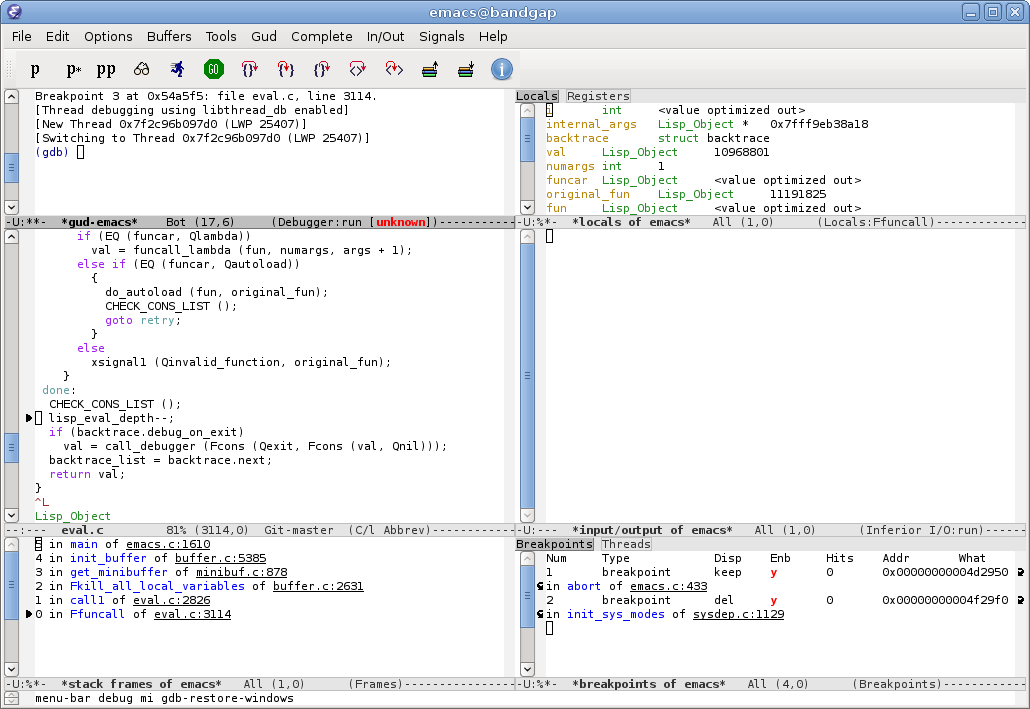
\includegraphics[height=.9\paperheight]{emacs-gdb.png}
  \end{centering}
\end{frame}


\begin{frame}[fragile]
  \frametitle{GDB в составе IDE}
  \begin{itemize}
  \item При работе через Machine Interface (\code{gdb -i=mi})
    информация выдаётся в структурированном виде
\begin{lstlisting}[style=session]
(gdb) -stack-info-frame
^done,frame={level="0",
             addr="0x0804888f",func="main",
             file="stl.c",
             fullname="/home/dzhus/stl.c",
             line="10"}
\end{lstlisting}
  \item GDB уведомляет клиента об изменениях состояния
\begin{lstlisting}[style=session]
=thread-created,id="6",group-id="22226"
*running,thread-id="6"
\end{lstlisting}
  \end{itemize}
\end{frame}

\begin{frame}
  \frametitle{Чего не хватало в Emacs}
  \begin{itemize}
  \item Ранее Emacs использовал устарейвший командный интерфейс
    «с аннотациями»
  \item Не было поддержки безостановочной отладки
  \item Кто, если не мы?
  \end{itemize}
\end{frame}

\section{GSoC}
\begin{frame}
  \frametitle{Google Summer of Code}
  \begin{columns}
    \column{.3\textwidth}
    \cenfig{0.1}{google.jpg}
    \column{.7\textwidth}
  \begin{itemize}
  \item Международная летняя программа для студентов
  \item Под руководством ментора из числа опытных разработчиков
    студент работает над проектом в области свободного \textsc{ПО}
  \item С 2005 года в программе успешно приняли участие 2500 студентов
    из 98 стран
  \end{itemize}
\end{columns}
\end{frame}

\begin{frame}
  \frametitle{Как устроена программа GSoC}
  \begin{itemize}
  \item В начале года \neword{организации} подают заявки на участие,
    на основе которых их принимают в программу и распределяют слоты
    для участников
  \item В марте \neword{студенты} подают заявки с описанием своих
    \neword{проектов}, которые рассматриваются организациями
  \item На основе заявок определяется список студентов, которые будут
    участвовать в программе, назначаются \neword{менторы}
  \item Основная работа начинается в конце мая
  \item В середине июля — \neword{смотр}
  \item Проекты проходят \neword{финальный смотр} в середине августа
  \end{itemize}
\end{frame}

\subsection{Проект «GDB/MI Emacs migration»}
\begin{frame}
  \frametitle{Основные достижения}
  \begin{itemize}
  \item Emacs-интерфейс к GDB полностью переведён на MI
  \item За счёт перехода на MI теперь поддерживается безостановочная
    отладка и просмотр разных нитей/фреймов одновременно
  \item Множественные улучшения и рефакторинг кода
    \begin{itemize}
    \item JSON-парсер вместо регулярных выражений
    \item Снижено связывание за счёт использования модели с оповещениями
      для обновления информации в буферах IDE
    \end{itemize}
  \end{itemize}
\end{frame}

\begin{frame}[fragile]
  \frametitle{«Нет» регулярным выражениям}
  \begin{itemize}
  \item JSON — простой и гибкий формат обмена структурированными
    данными (объекты с полями + списки)
  \item Формат ответов MI хорошо ложится на модель JSON
    \begin{itemize}
    \item \textbf{MI}
\begin{lstlisting}
locals=[{name="threads", type="pthread_t [5]"},
        {name="i", type="int",value="3"}]
\end{lstlisting}

    \item \textbf{JSON}
\begin{lstlisting}
{"locals":[{"name":"threads", 
            "type":"pthread_t [5]"},
           {"name":"i", 
            "type":"int", 
            "value":"3"}]}
\end{lstlisting}
    \end{itemize}
  \item Использовать рег. выражения для разбора MI неудобно и
    неправильно (КС-грамматика)
  \end{itemize}
\end{frame}

\begin{frame}[fragile]
  \frametitle{MI в Lisp}
  \begin{itemize}
  \item MI тривиально переводится в JSON, после чего разбирается
    JSON-парсером
    \begin{itemize}
    \item \textbf{MI}
\begin{lstlisting}
locals=[{name="threads", type="pthread_t [5]"},
        {name="i", type="int",value="3"}]
\end{lstlisting}
    \item \textbf{Lisp}
\begin{lstlisting}
((locals .
         [((type . "pthread_t [5]")
           (name . "threads"))
          ((value . "3")
           (type . "int")
           (name . "i"))]))
\end{lstlisting}
    \end{itemize}

  \item Работать с естественными Лисп-структурами проще, чем с
    результатами применения регулярных выражений
  \end{itemize}
\end{frame}

\begin{frame}[fragile]
  \frametitle{Pub \& sub}
  \begin{itemize}
  \item Буфер каждого типа обновлялся явным образом: расходы на поиск
    и недостаточная гибкость
    \begin{columns}
      \column{.4\textwidth}
      \begin{figure}[h]
        \centering
        \begin{tikzpicture}[style=tight]
          \node at (0, 0) [rectangle] (phantom) {\phantom{updater}};
          \node at ($ (phantom) + (0, -1) $)
          [draw=red!50!black, thick, rectangle, rounded corners=2pt] (updater) {updater};
          
          \foreach \an / \num in {-1/1, 0/2, 1/3} { \draw node at
            ($ (updater.south) + (\an,-1) $)
            [draw, circle] (b\num) {$\mathbf{b_\num}$};
            
            \draw[->] (updater) to (b\num); 
          }
        \end{tikzpicture}
        
        \color{red!50!black}{Было}
      \end{figure}
      \begin{lstlisting}[language=Lisp]
(defun gdb-update ()
  (update-locals)
  (update-registers)
  ...)
\end{lstlisting}
      \column{.4\textwidth}
      \begin{figure}[h]
        \centering
        \begin{tikzpicture}[style=tight]
          \node at (0, 0) [draw, rectangle] (updater) {updater};
          
          \node at ($ (updater) + (0, -1) $) 
          [draw=green!50!black, thick, rectangle, rounded corners=2pt] (pub)  {publisher};
          
          \draw[->] (updater) -- (pub); 
          
          \foreach \an / \num in {-1/1, 0/2, 1/3} { \draw node at
            ($ (pub.south) + (\an,-1) $)
            [draw, circle] (b\num) {$\mathbf{b_\num}$};
            
            \draw[->, dashed] (pub) to (b\num); 
          }
        \end{tikzpicture}
        
        \color{green!50!black}{Стало}
      \end{figure}
      \begin{lstlisting}[language=Lisp]
(defun gdb-update ()
  (emit-signal 
   buf-publisher
   'update))
      \end{lstlisting}
    \end{columns}
  \end{itemize}
\end{frame}

\begin{frame}[fragile]
  \frametitle{Опыт GSoC}
  \begin{itemize}
  \item Обсуждения в рассылках для разработчиков GDB и Emacs и в {\tt
      comp.lang.lisp}
  \item Прямой доступ к Emacs CVS
  \item Рабочий процесс: личный Mercurial плюс upstream CVS.
  \item Потребовалось больше рефакторинга, чем казалось сначала

  \item Объём выполненных работ:
    \begin{itemize}
    \item 285 коммитов
    \item Общие изменения {\color{green!50!black}6915 (+)},
      {\color{red!50!black}3994 (-)}
    \item Итоговые изменения {\color{green!50!black}2390 (+)},
      {\color{red!50!black}802 (-)}
    \end{itemize}

  \end{itemize}
\end{frame}

\begin{frame}
  \frametitle{Tips \& Tricks}
  \begin{itemize}
  \item Начинать общаться со своей организацией \emph{до} начала программы
    
  \item Заявка на участие должна отражать готовность работать

  \item План работ помогает разобраться в задаче
    
  \item Постоянная работа с собственными мыслями и наблюдениями
    
  \item Взаимодействие с сообществом!

  \item Это \emph{не} соревнование
  \end{itemize}
\end{frame}

\appendix
\begin{frame}
  \frametitle{О чём был доклад}
  \begin{itemize}
  \item Свободный отладчик GDB развивается и отвечает на вызовы
    времени
  \item Лето с Google — прекрасная возможность получить опыт и
    принести пользу сообществу и себе
  \end{itemize}
\end{frame}
\end{document}